\begin{table}
\caption{Overview of assimilation experiments performed.}
\centering
\begin{tabular}{p{2cm}p{2cm}p{6cm}p{4cm}}
	Experiment& Model &  Assimilated Quantities  & Run dates \\
\hline
E1 & CAM	&	none &  1 Jan - 28 Feb 2009 \\
E2 & CAM &	$\chi_1$, $\chi_2$, $\Delta$LOD	& 1 Jan - 28 Feb 2009 \\
E3 & CAM &	Radiosonde temperatures	& 1 Jan -31 Jan 2009	\\
E4 & CAM &	Radiosonde temperatures, $\chi_1$, $\chi_2$, $\Delta$LOD	& 1 Jan - 17 Jan 2009\\
E5 & WACCM &	none   & 1-30 Oct 2009	\\
E6 & WACCM &	GPS-RO + NNRA$^b$ tropics only & 1-30 Oct 2009	\\
E7 & WACCM &	GPS-RO + NNRA$^b$ whole atmosphere  & 1-30 Oct 2009	\\
E8$^a$ & WACCM &	GPS-RO + NNRA$^b$ whole atmosphere +SABER & 1 Jan - 28 Feb 2009\\	
\hline
\end{tabular}
\tablenotetext{a}{Experiments performed by \citet{Pedatella2014}}
\tablenotetext{b}{Observations used in the NCEP/NCAR Reanalysis project \citet{Saha2010}, which include radiosonde and aircraft winds and temperatures, plus satellite drift winds.}
\label{tab:expts}
\end{table}
\clearpage


%------comparison of the DA runs in the observation space
\begin{figure}[p]
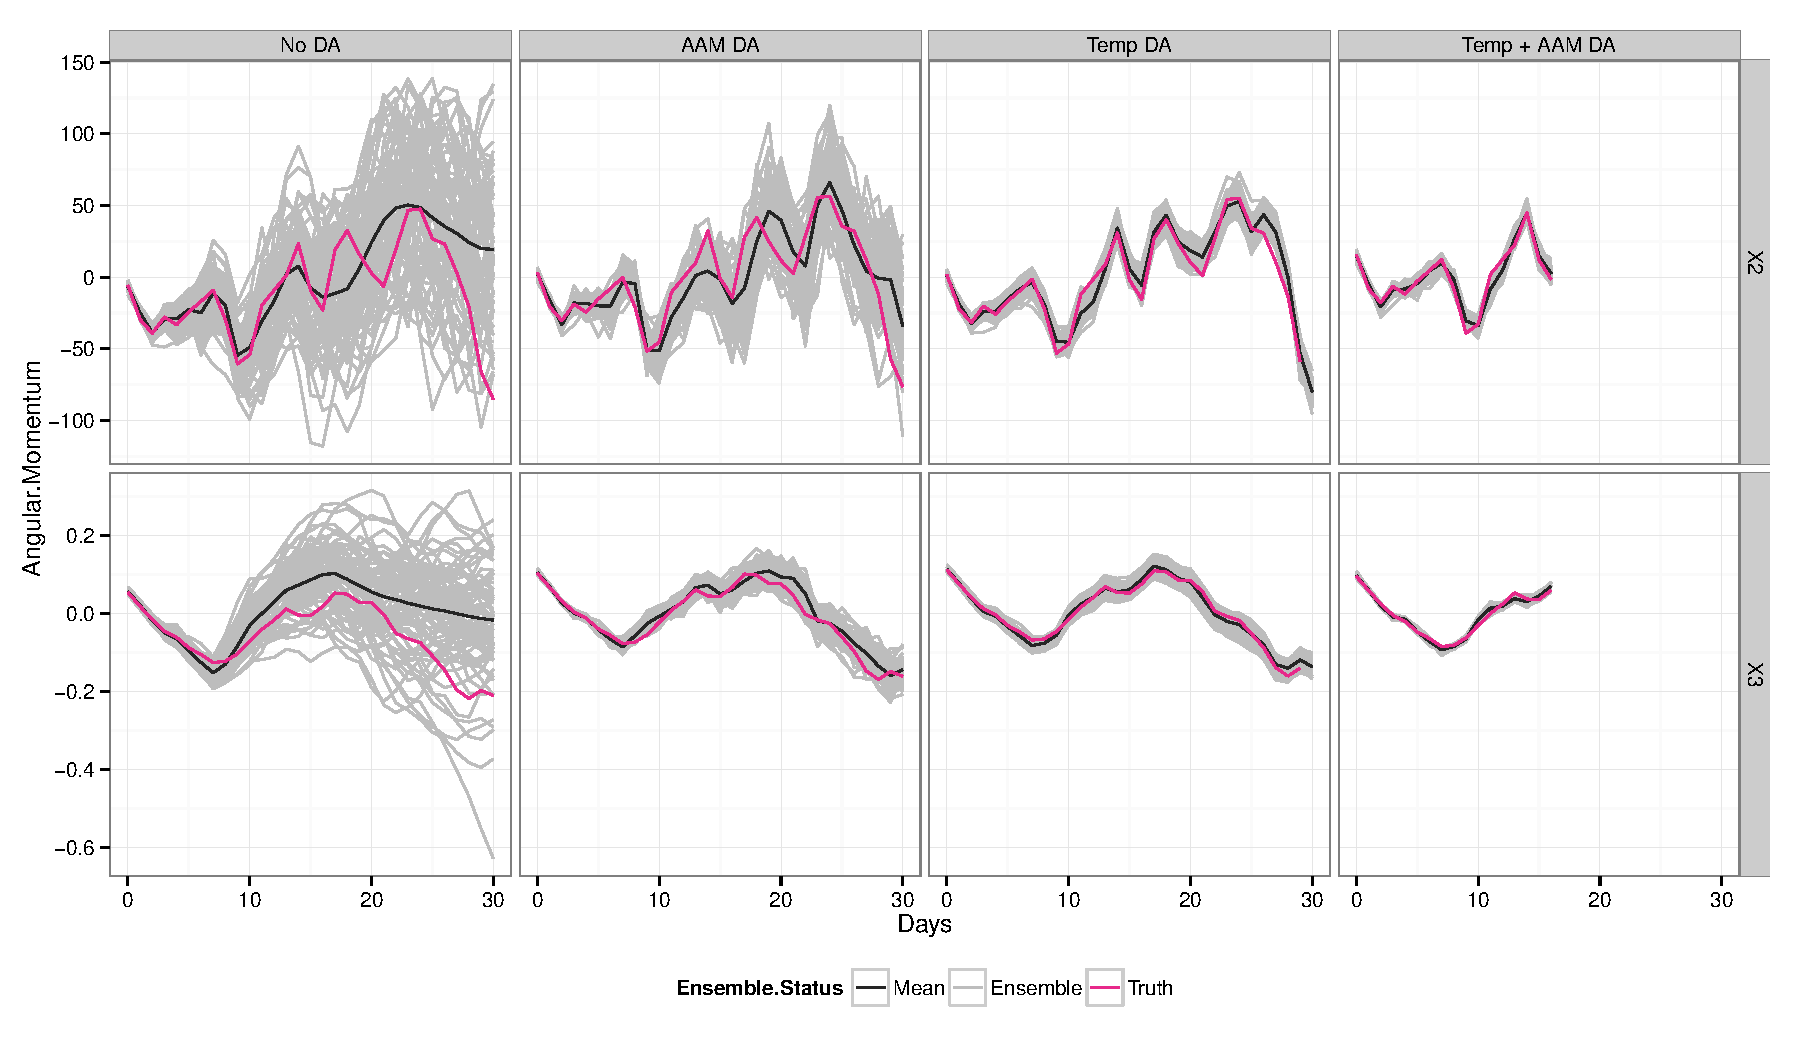
\includegraphics[width=\textwidth]{Paper_figures/ERPDA_paper_erpda_obs_space.pdf} 
 \caption{ The DART prior ensemble (gray) compared to the true state (green) in terms of assimilation time and each of the three angular momentum functions [(\ref{eq:X1})-(\ref{eq:X3}), (\ref{eq:X3_to_LOD})].  The columns compare the four experiments summarized in Table \ref{tab:expts}.  }
 \label{fig:fit_to_ERPs}
\end{figure}

%-----evolution of the covariances between local variables and the AAM observations 
 \begin{figure}
	 \includegraphics[width=\textwidth]{Paper_figures/ERPDA_paper_U_to_LOD_covariances.pdf}
	 \caption{Evolution of the covariance zonal wind and the axial angular momentum component ($\chi_3$) on three dates in E2 (assimilating AAM). The top row shows values averaged over stratospheric levels, while the bottom row shows values averaged over tropospheric levels.}
 \label{fig:covariances}
\end{figure}

%-----evolution of the prior error and corresponding increments 
 \begin{figure}
	 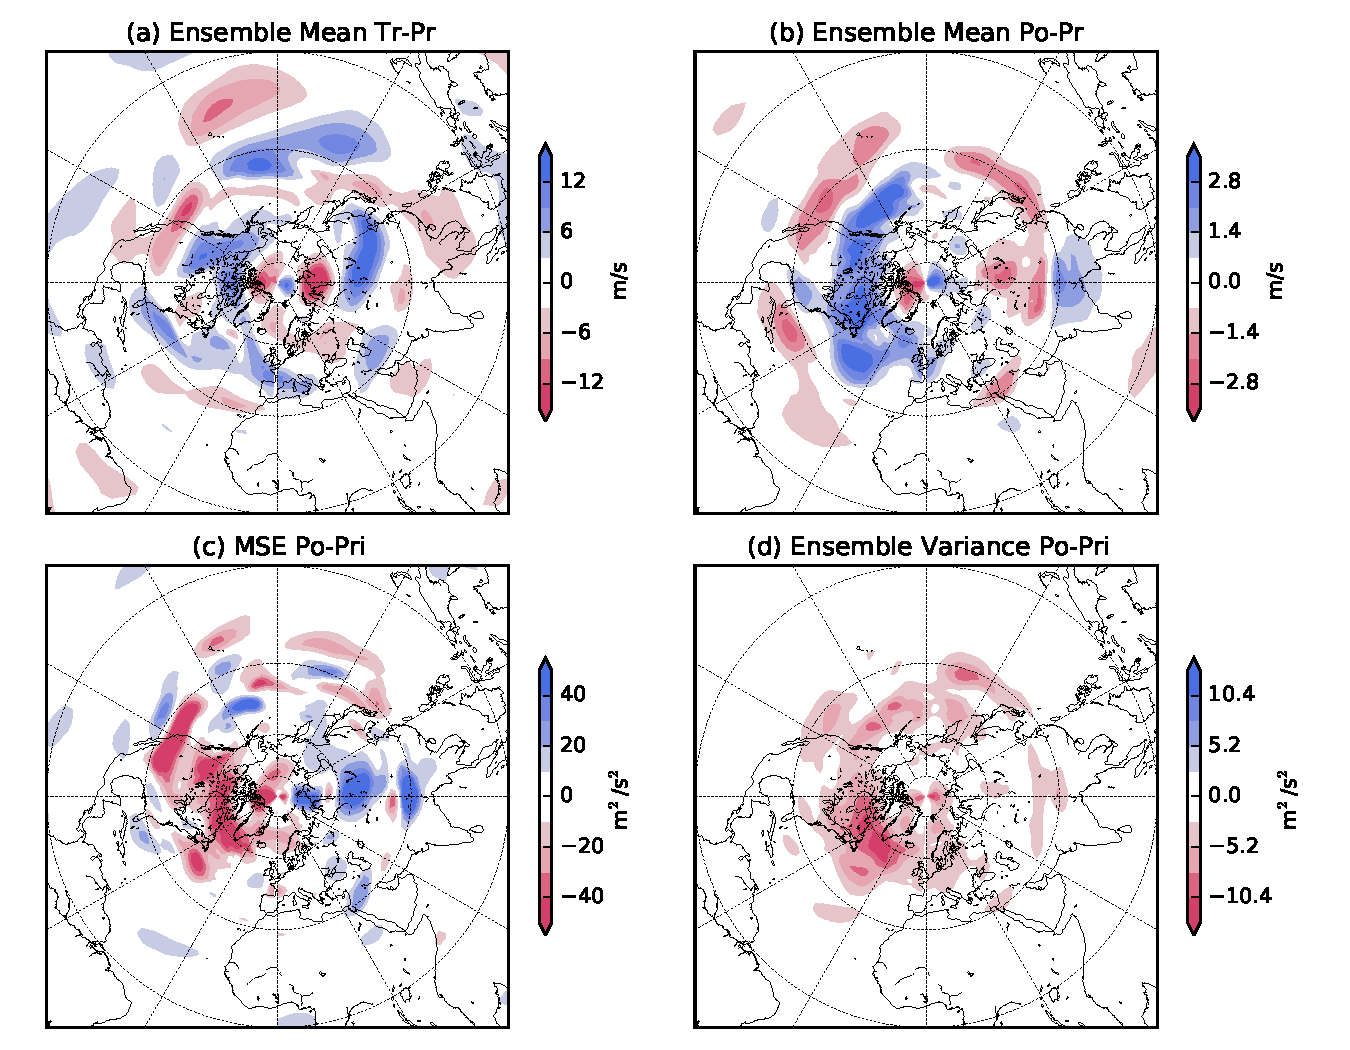
\includegraphics[width=\textwidth]{Paper_figures/ERPDA_paper_U_priorerror_vs_increment_vs_ER_31jan.pdf}
	 \caption{Snapshots of the (a) bias (truth minus prior ensemble mean), (b) analysis increment (posterior minus prior ensemble mean), (c) posterior minus prior mean square error, and (d) posterior-minus prior ensemble variance on 31 January, i.e. after 1 month of assimilation, on the 320 hPa vertical leve, and all for assimilation in experiment E2 (assimilating AAM only). } 
 \label{fig:error_increments}
\end{figure}


%-----focus on the ensemble in two regions to show how it is moved away from the true state
 \begin{figure}
	 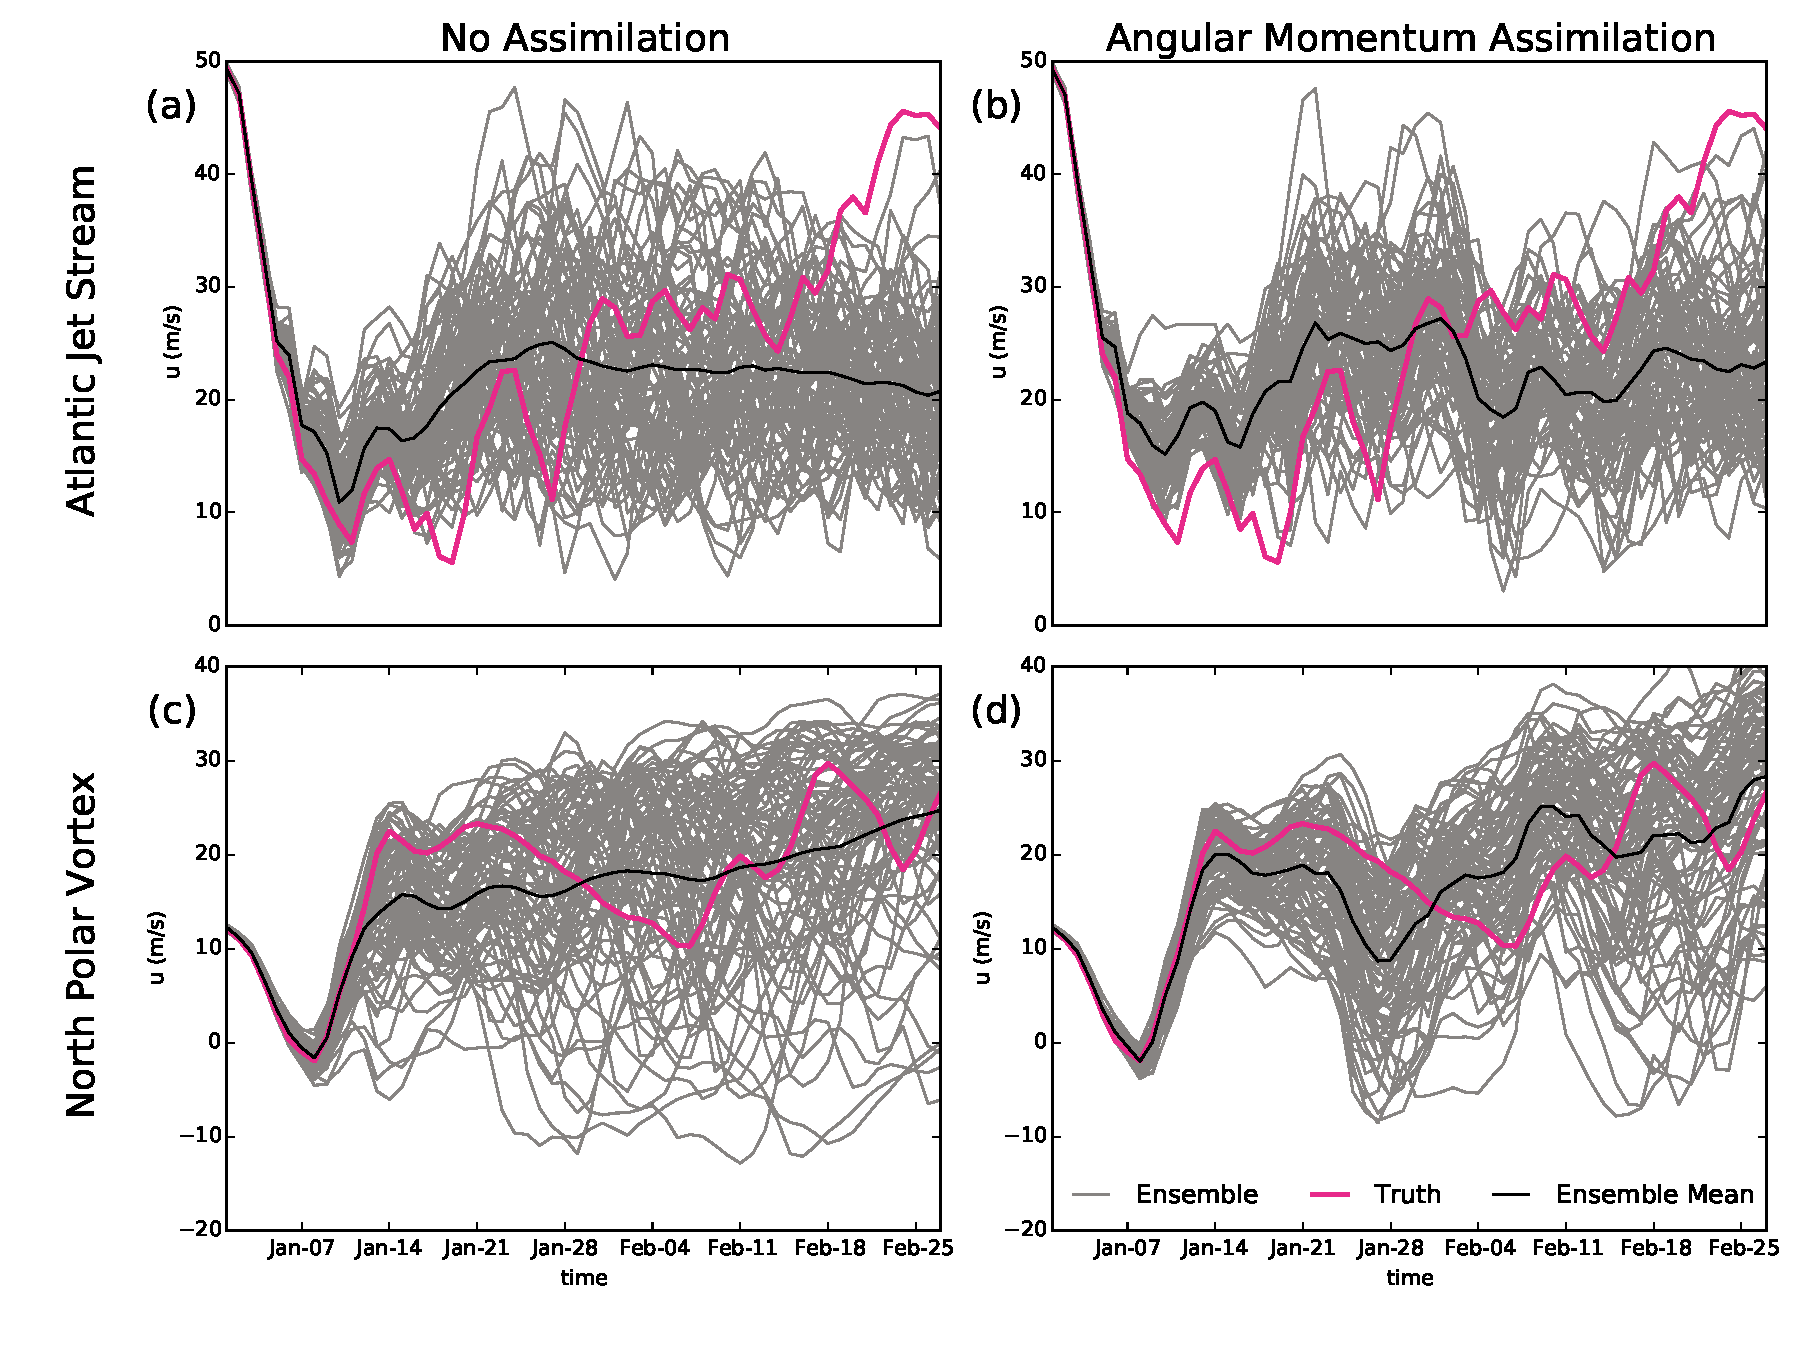
\includegraphics[width=\textwidth]{Paper_figures/ERPDA_paper_point_checks.pdf}
	 \caption{Comparison of the ensemble (gray) and its mean (black) to the true state (pink), for no assimilation (left column) and with assimilation of the three angular momentum components (right column). The top row shows zonal wind averaged over the North Atlantic jet (see text), and the bottom row shows zonal wind averaged in the polar vortex (see text).}
	 \label{fig:point_checks}
\end{figure}




%------difference in MSE for RST - ERPRST (blue is good)
 \begin{figure}
	 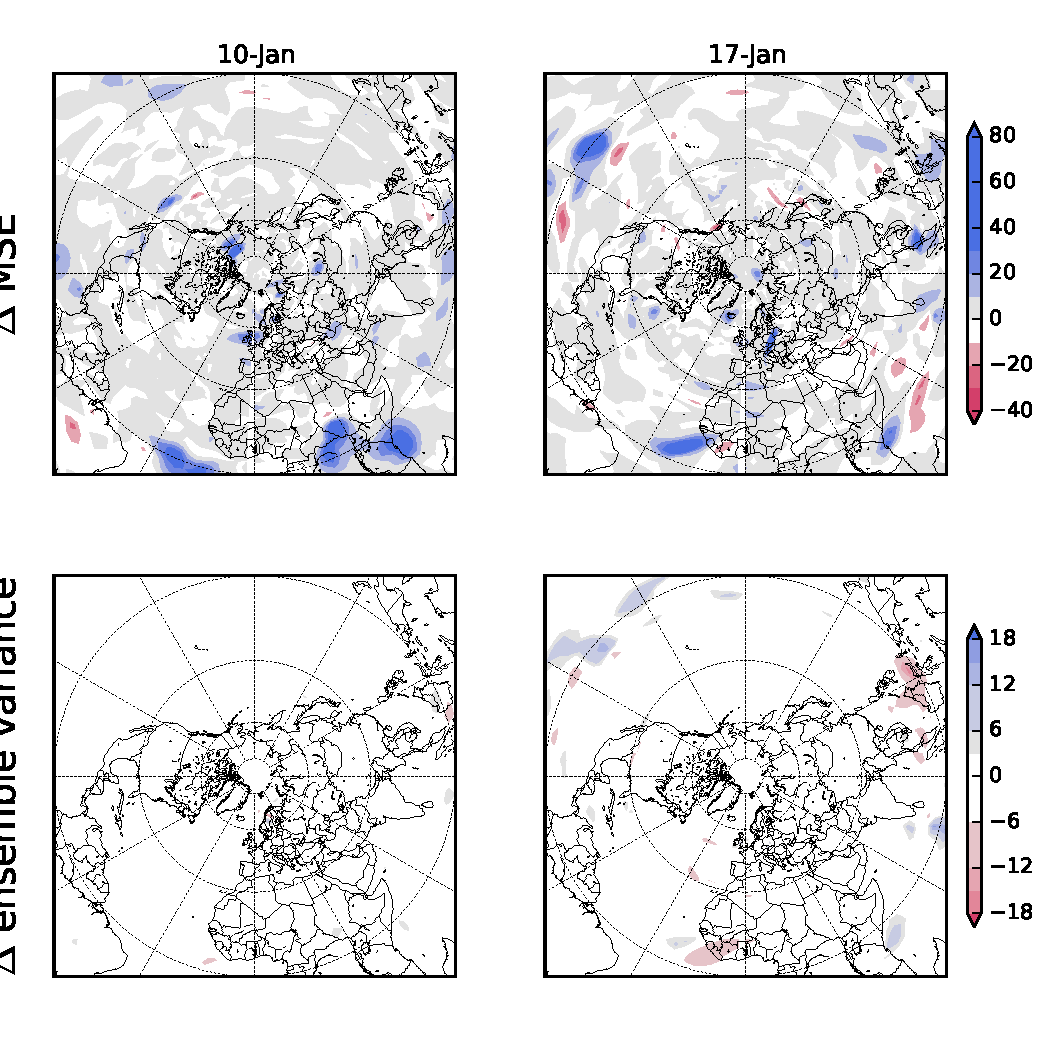
\includegraphics[width=\textwidth]{Paper_figures/ERPDA_paper_U_error_RST_vs_ERPRST.pdf}
	 \caption{Snapshots of the difference in mean square error (top) and scaled ensemble variance (see eqn \ref{eq:EvsS}) (bottom) between the assimilation of radiosonde temperatures and the assimilation of both radiosonde temperatures and the global angular momentum, averaging between the surface and 100 hPa. Blue indicates that adding the angular momentum to the assimilation reduces error / ensemble variance. }
	 \label{fig:added_value_MSE}
\end{figure}

%-----evolution of rank histograms to show filter divergence when you add ERPs to RST  
 \begin{figure}
	 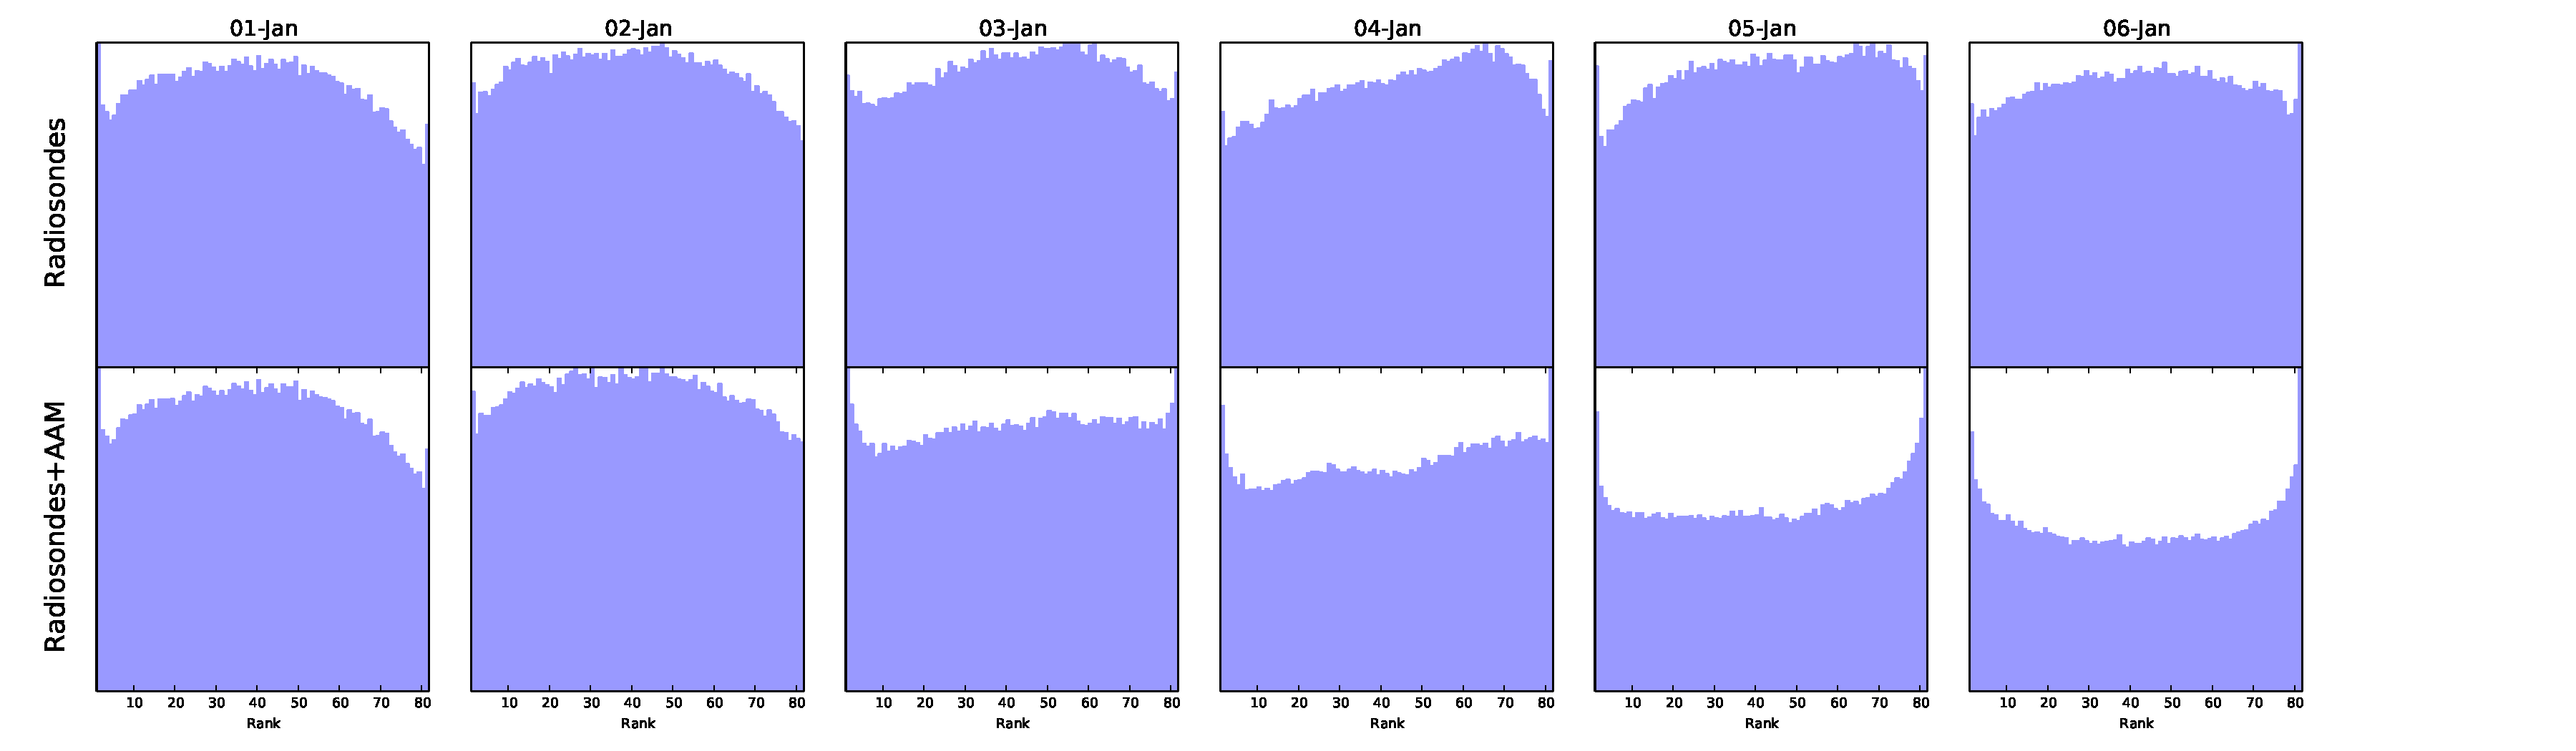
\includegraphics[width=\textwidth]{Paper_figures/ERPDA_paper_added_value_RH.pdf}
	 \caption{Evolution of the rank histogram of the zonal wind field over the first week of assimilation of (top) radiosonde temperatures and (bottom) radiosonde temperatures with angular momentum.}
	 \label{fig:added_value_RH}
\end{figure}

%-------comparison of the WACCM experiments in terms of true error ----
 \begin{figure}
	 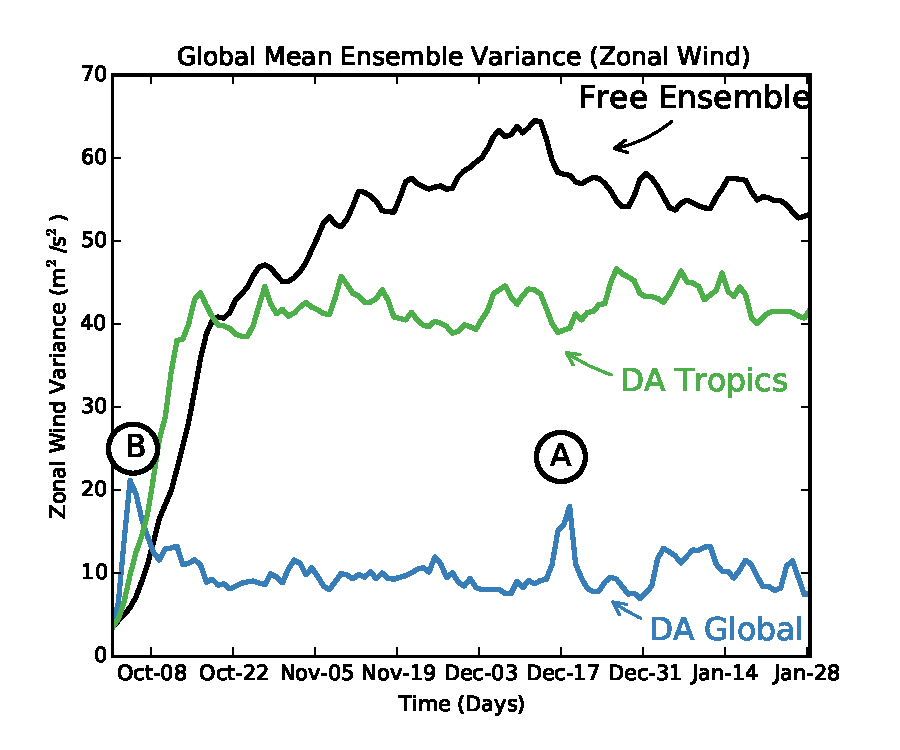
\includegraphics[width=\textwidth]{Paper_figures/ERPDA_paper_evalvariable_state_space.pdf}
	 \caption{Global-average ensemble variance as a function of time, for experiments E5-E8, which all assimilated real observations into WACCM using DART.}
	 \label{fig:evalvariable_state}
\end{figure}



%-------comparison of the WACCM experiments in terms of aam ----
\begin{figure}
	 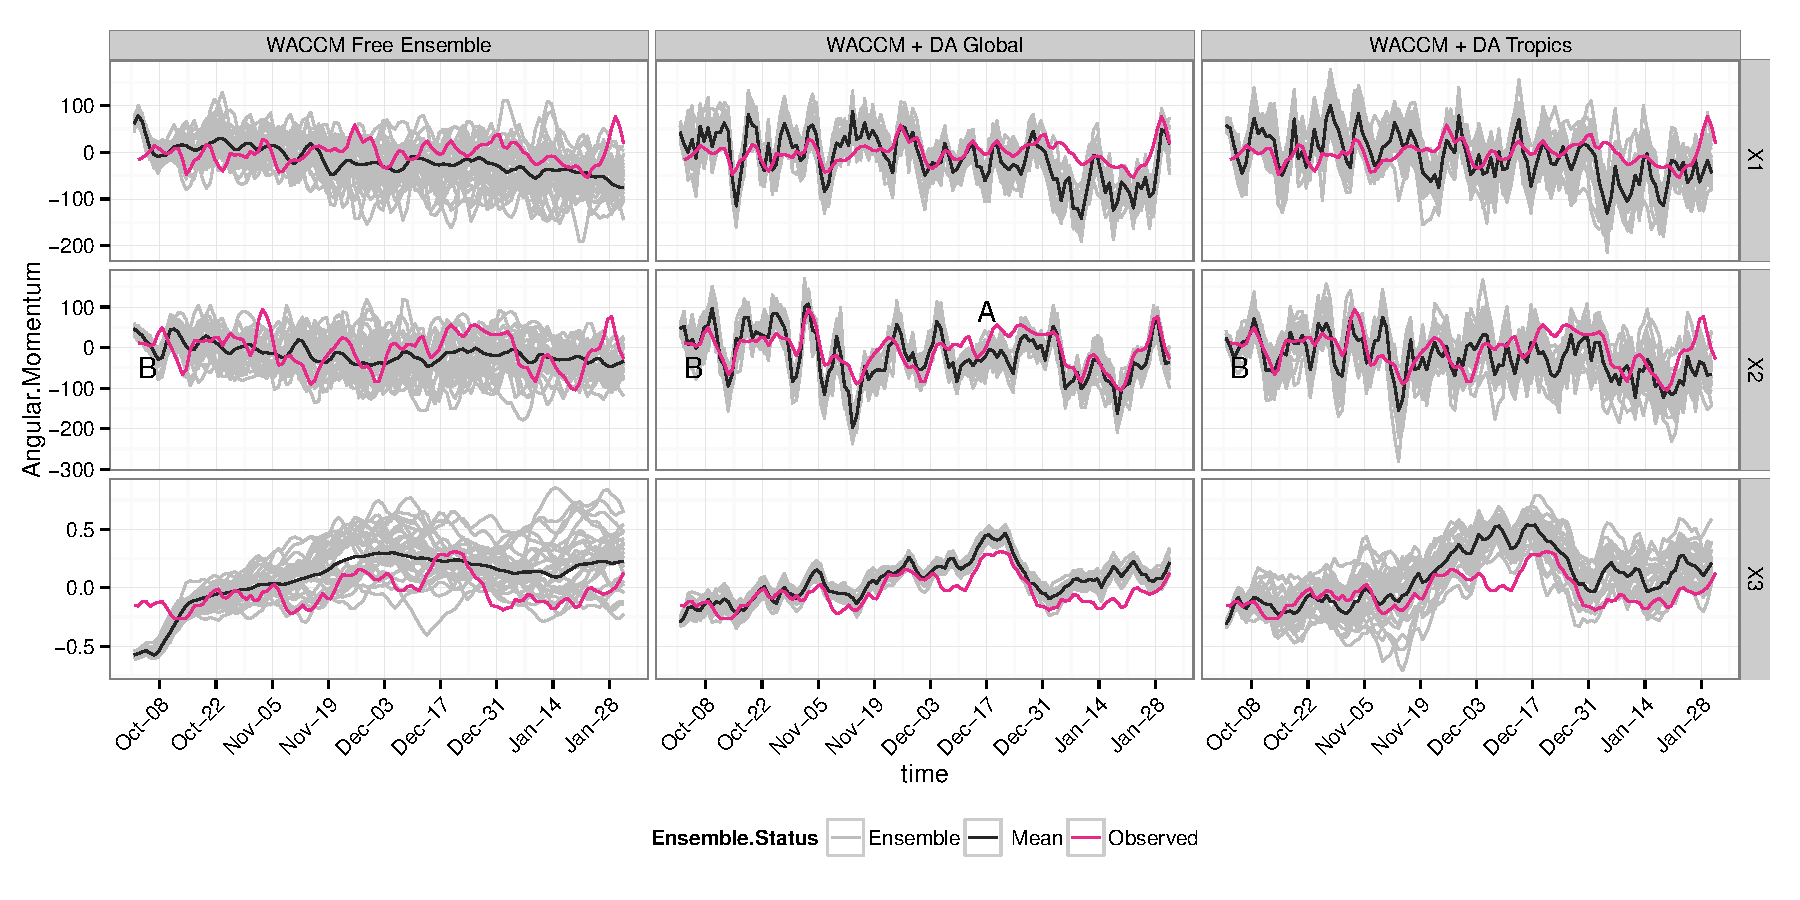
\includegraphics[width=0.8\textwidth]{Paper_figures/ERPDA_paper_evalvariable_aam_space.pdf}
	 \caption{Comparison of the ensemble (gray) in experiments E5-E8, in terms of their axial angular momentum excitation functions $\chi_3$, scaled to equivalent length-of-day anomalies using (\ref{eq:X3_to_LOD}), and compared to the observed anomalous length-of-day for each case.}
	 \label{fig:evalvariable_aam}
\end{figure}





